

\begin{frame}
  \frametitle{Kernel-PCA}
  
  \begin{block}{Principle: non linear transformation of $\bx$ before PCA} 
    \begin{enumerate}
      \item Project the data into a higher space where it is linearly separable
      \item Apply PCA to the transformed data 
    \end{enumerate}
  \end{block}

  \begin{figure}[ht]
    \centering
    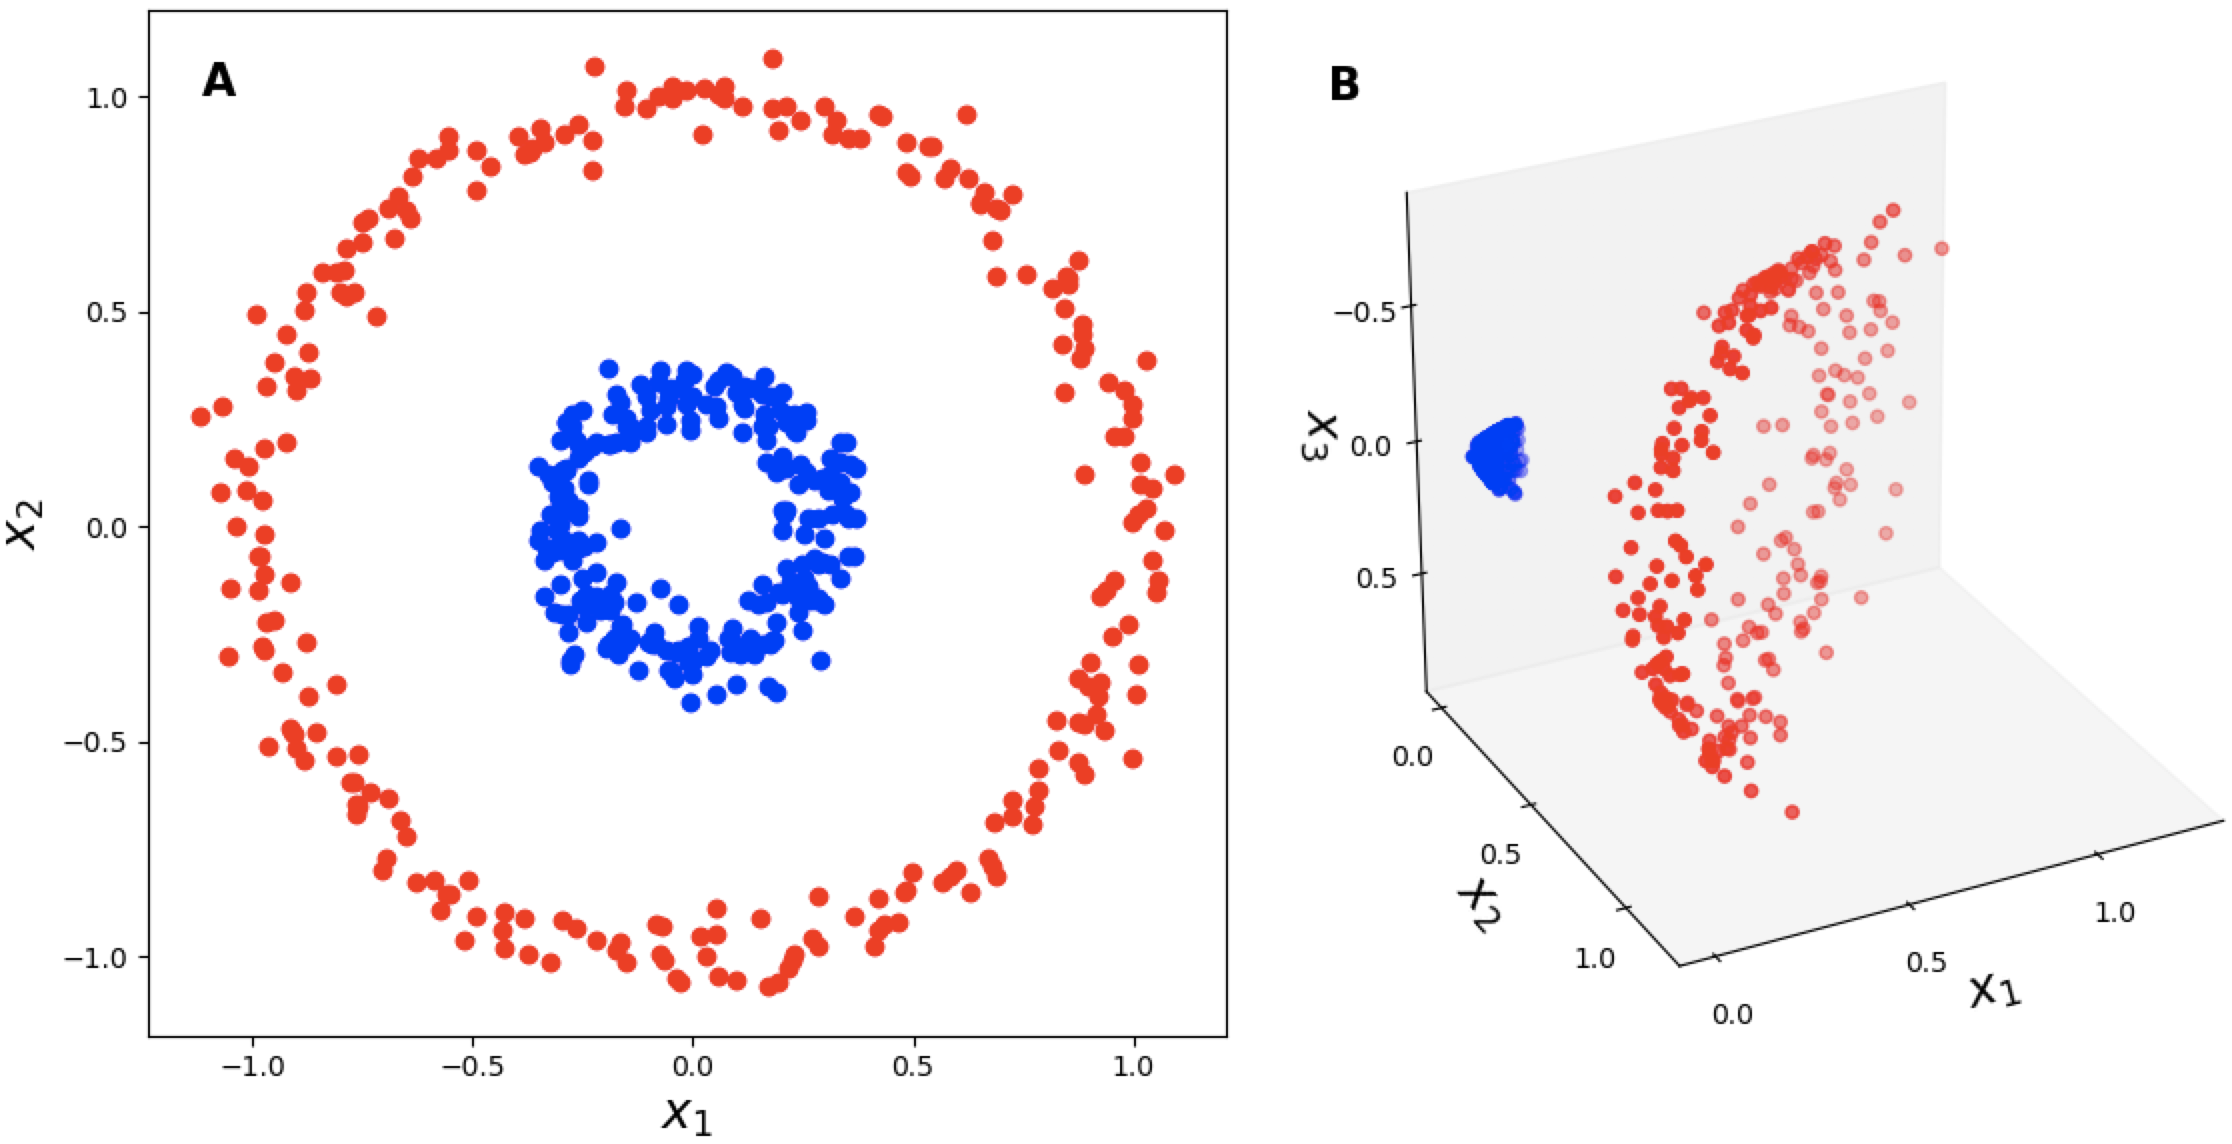
\includegraphics[height=4cm]{figures/kernel_trick2}
    \caption{$\Psi : \bx \to \Psi(\bx)$}
  \end{figure}

\end{frame}

\begin{frame}
  \frametitle{Kernel-PCA}

  \begin{block}{Kernel PCA Model}
    Assume a non linear transformation $ \Psi(\mathbf{x}_i) \text{ where } \Psi : \mathbb{R}^p \to \mathbb{R}^n$,  then perform linear PCA, with $\bV$ a \alert{\bf $n\times q$} orthonormal matrix
    \[
      \Phi(\bx) = \bV^\top \Psi(\bx-\bmu) = \tilde\bx
    \]
  \end{block}

  \begin{block}{Kernel trick}
    Never calculate  $\Psi(\bx_i)$ thanks to the kernel trick:
    \[K = k(\mathbf{x},\mathbf{y}) = (\Psi(\mathbf{x}),\Psi(\mathbf{y})) = \Psi(\mathbf{x})^T\Psi(\mathbf{y}) \]
  \end{block}

  \begin{block}{Solution}
    Eigen-decomposition of the doubly centered kernel matrix $\mathbf{K} = k(\bx_i, \bx_{i'})$ 
    \[\tilde{\mathbf{K}} = 
    (\bI - \mathbf{1}\mathbf{1}^\top/n) \mathbf{K} (\bI - \mathbf{1}\mathbf{1}^\top/n) = \bV {\boldsymbol\Lambda} \bV^\top \]
  \end{block}

\end{frame}

\begin{frame}[fragile]
  \frametitle{Choice of a kernel} 

  $k(\mathbf{x},\mathbf{y})$ 

  Depends on the kind of similarity you assume 

\begin{block}{Some common kernels}

\begin{itemize}
\item \alert{\bf Polynormial Kernel }

\[ k(\bx_i,\bx_{i'}) = (\bx_{i}^\top \bx_{i'} + c)^d \]

\item  \alert{\bf Gaussian (radial) kernel}

\[k(\bx_i,\bx_{i'}) = exp{\frac {-\left\|\bx_i - \bx_{i'} \right\|^2}{2\sigma^2}\]

\item  \alert{\bf Laplacian kernel}

\[k(\bx_i,\bx_{i'}) = exp{\frac {-\left\|\bx_i - \bx_{i'} \right\|}{\sigma}\]

\end{block}

\rsa Kernel PCA suffers from the choice of the Kernel to correctly

\end{frame}


\begin{frame}[fragile]
  \frametitle{Example on scRNA} 
  \framesubtitle{Run the fit}

\begin{knitrout}
\definecolor{shadecolor}{rgb}{0.969, 0.969, 0.969}\color{fgcolor}\begin{kframe}
\begin{alltt}
\hlstd{scRNA_expr} \hlkwb{<-} \hlstd{scRNA} \hlopt \hlkwd{select}\hlstd{(}\hlopt{-}\hlstd{cell_type)} \hlopt \hlkwd{as.matrix}\hlstd{()}
\end{alltt}


{\ttfamily\noindent\bfseries\color{errorcolor}{\#\# Error in scRNA \%>\% select(-cell\_type) \%>\% as.matrix(): could not find function "{}\%>\%"{}}}\begin{alltt}
\hlstd{kPCA_radial} \hlkwb{<-}
  \hlkwd{kpca}\hlstd{(scRNA_expr,} \hlkwc{kernel} \hlstd{=} \hlstr{"rbfdot"}\hlstd{,} \hlkwc{features} \hlstd{=} \hlnum{2}\hlstd{,} \hlkwc{kpar} \hlstd{=} \hlkwd{list}\hlstd{(}\hlkwc{sigma} \hlstd{=} \hlnum{0.5}\hlstd{))} \hlopt
  \hlkwd{pcv}\hlstd{()} \hlopt \hlkwd{as.data.frame}\hlstd{()} \hlopt
  \hlkwd{add_column}\hlstd{(}\hlkwc{kernel} \hlstd{=} \hlstr{"Radial"}\hlstd{)} \hlopt
  \hlkwd{add_column}\hlstd{(}\hlkwc{cell_type} \hlstd{= scRNA}\hlopt{$}\hlstd{cell_type)}
\end{alltt}


{\ttfamily\noindent\bfseries\color{errorcolor}{\#\# Error in kpca(scRNA\_expr, kernel = "{}rbfdot"{}, features = 2, kpar = list(sigma = 0.5)) \%>\% : could not find function "{}\%>\%"{}}}\begin{alltt}
\hlstd{kPCA_linear} \hlkwb{<-}
  \hlkwd{kpca}\hlstd{(scRNA_expr,} \hlkwc{kernel} \hlstd{=} \hlstr{"vanilladot"}\hlstd{,} \hlkwc{features} \hlstd{=} \hlnum{2}\hlstd{,} \hlkwc{kpar} \hlstd{=} \hlkwd{list}\hlstd{())} \hlopt
  \hlkwd{pcv}\hlstd{()} \hlopt \hlkwd{as.data.frame}\hlstd{()} \hlopt
  \hlkwd{add_column}\hlstd{(}\hlkwc{kernel} \hlstd{=} \hlstr{"Linear"}\hlstd{)} \hlopt
  \hlkwd{add_column}\hlstd{(}\hlkwc{cell_type} \hlstd{= scRNA}\hlopt{$}\hlstd{cell_type)}
\end{alltt}


{\ttfamily\noindent\bfseries\color{errorcolor}{\#\# Error in kpca(scRNA\_expr, kernel = "{}vanilladot"{}, features = 2, kpar = list()) \%>\% : could not find function "{}\%>\%"{}}}\begin{alltt}
\hlstd{kPCA_polydot} \hlkwb{<-} \hlkwd{kpca}\hlstd{(scRNA_expr,} \hlkwc{kernel} \hlstd{=} \hlstr{"polydot"}\hlstd{,} \hlkwc{features} \hlstd{=} \hlnum{2}\hlstd{,} \hlkwc{kpar} \hlstd{=} \hlkwd{list}\hlstd{(}\hlkwc{degree} \hlstd{=} \hlnum{3}\hlstd{))} \hlopt
  \hlkwd{pcv}\hlstd{()} \hlopt \hlkwd{as.data.frame}\hlstd{()} \hlopt
  \hlkwd{add_column}\hlstd{(}\hlkwc{kernel} \hlstd{=} \hlstr{"Polynomial"}\hlstd{)} \hlopt
  \hlkwd{add_column}\hlstd{(}\hlkwc{cell_type} \hlstd{= scRNA}\hlopt{$}\hlstd{cell_type)}
\end{alltt}


{\ttfamily\noindent\bfseries\color{errorcolor}{\#\# Error in kpca(scRNA\_expr, kernel = "{}polydot"{}, features = 2, kpar = list(degree = 3)) \%>\% : could not find function "{}\%>\%"{}}}\begin{alltt}
\hlstd{kPCA_laplacedot} \hlkwb{<-} \hlkwd{kpca}\hlstd{(scRNA_expr,} \hlkwc{kernel} \hlstd{=} \hlstr{"laplacedot"}\hlstd{,} \hlkwc{features} \hlstd{=} \hlnum{2}\hlstd{)} \hlopt
  \hlkwd{pcv}\hlstd{()} \hlopt \hlkwd{as.data.frame}\hlstd{()} \hlopt
  \hlkwd{add_column}\hlstd{(}\hlkwc{kernel} \hlstd{=} \hlstr{"Laplace"}\hlstd{)} \hlopt
  \hlkwd{add_column}\hlstd{(}\hlkwc{cell_type} \hlstd{= scRNA}\hlopt{$}\hlstd{cell_type)}
\end{alltt}


{\ttfamily\noindent\bfseries\color{errorcolor}{\#\# Error in kpca(scRNA\_expr, kernel = "{}laplacedot"{}, features = 2) \%>\% pcv() \%>\% : could not find function "{}\%>\%"{}}}\end{kframe}
\end{knitrout}
\end{frame}

\begin{frame}[fragile]
  \frametitle{Example on scRNA} 
  \framesubtitle{Compare the projection}

\begin{knitrout}
\definecolor{shadecolor}{rgb}{0.969, 0.969, 0.969}\color{fgcolor}\begin{kframe}
\begin{alltt}
\hlkwd{rbind}\hlstd{(kPCA_linear, kPCA_polydot, kPCA_radial, kPCA_laplacedot)} \hlopt
  \hlkwd{ggplot}\hlstd{(}\hlkwd{aes}\hlstd{(}\hlkwc{x} \hlstd{= V1,} \hlkwc{y} \hlstd{= V2,} \hlkwc{color} \hlstd{= cell_type))} \hlopt{+}
  \hlkwd{geom_point}\hlstd{(}\hlkwc{size}\hlstd{=}\hlnum{1.25}\hlstd{)} \hlopt{+} \hlkwd{guides}\hlstd{(}\hlkwc{colour} \hlstd{=} \hlkwd{guide_legend}\hlstd{(}\hlkwc{override.aes} \hlstd{=} \hlkwd{list}\hlstd{(}\hlkwc{size}\hlstd{=}\hlnum{6}\hlstd{)))} \hlopt{+}
  \hlkwd{facet_wrap}\hlstd{(.}\hlopt{~}\hlstd{kernel,} \hlkwc{scales} \hlstd{=} \hlstr{'free'}\hlstd{)} \hlopt{+} \hlkwd{labs}\hlstd{(}\hlkwc{x} \hlstd{=} \hlstr{''}\hlstd{,} \hlkwc{y} \hlstd{=} \hlstr{''}\hlstd{)}
\end{alltt}


{\ttfamily\noindent\bfseries\color{errorcolor}{\#\# Error in rbind(kPCA\_linear, kPCA\_polydot, kPCA\_radial, kPCA\_laplacedot) \%>\% : could not find function "{}\%>\%"{}}}\end{kframe}
\end{knitrout}

\end{frame}

